\chapter{Implementzione}

\lstnewenvironment{Code03_01}[1][]{\lstset{basicstyle=\small\ttfamily, columns=fullflexible,framexrightmargin=+.1\textwidth, keywordstyle=\color{red}\bfseries, commentstyle=\color{blue},language=C++, basicstyle=\small,  numberstyle=\tiny, stepnumber=1, numbersep=5pt, frame=shadowbox, #1}}{}


\chapter{Strumenti di sviluppo}
Lo sviluppo della nostra libreria ha richiesto l'uso di strumenti specifici atti a facilitare e sistematizzare la gestione del codice quali \texttt{git}, \texttt{CMake} e \texttt{Dxygen}.\\
\href{https://github.com/}{\texttt{Git}} è un sistema di controllo versione utilizzavile direttamente da linea di comando, molto diffuso è utile per tenere traccia delle varie fasi di sviluppo del codice. Git gestisce in modo adeguato i contributi al codice provenienti da agenti esterni e permette la condivisione del codice.\\
\href{http://www.cmake.org/}{\texttt{CMake}} è un software libero multipiattaforma nato per l'automazione dello sviluppo. Sostanzialmente con l'uso di \texttt{CMake} è possibile configurare e generare Makefile per il sistema operativo in uso. Questo facilita la diffusione del codice tra sviluppatori, non dovendo far altro che lanciare \texttt{CMake} e lasciare che sia lui ad occuparsi della ricerca di compilatori e librerie locali e della costruzione di software.\\
\href{www.doxygen.org/}{\texttt{Doxygen}} è un sistema multipiattaforma molto diffuso per la generazione automatica della documentazione di un codice. Per ottenere la documentazione è necessario introdurre nel codice dei commenti con una sintassi particolare, e il risultato è contiene l’elenco delle classi implementate, i loro diagrammi di collaborazione e la descrizione di metodi ed attributi.

\section{\texttt{Git}}
Il codice del progetto è reperibile su \texttt{git} ed è possibile scaricarlo e collabolare allo sviluppo clonando il codice dalla repository  \href{https://github.com/}{\texttt{GitHub}}:\\
\begin{center}
\texttt{ git clone https://github.com/mariaiemoli/progetto.git}
\end{center}
Nella cartella principale è contenuto anche un file \texttt{.gitignore}, in cui sono specificate le estensioni dei files e le sottocartelle che non devono essere visionati in una repository \texttt{git}. In particolare non si è interessati ai files temporanei che vengono eventualmente generati dagli editor, e alle cartelle generate da uno scorretta configurazione di \texttt{Doxygen}.

\section{\texttt{CMake}}
\texttt{CMake} si basa sulla creazione di files \texttt{CMakeLists.txt} nella directory del progetto, che contengono le direttive necessarie per creare il \texttt{Makefile} per compilare ed eseguire il codice. \\
Nella directory principale si trova un primo file \texttt{CMakeLists.txt} in cui si impostano i parametri fondamentali quali la dipendenza dalla versione di \texttt{CMake}, il nome del progetto, si includono le directory dei sorgenti nel path di compilazione e si caricano le librerie esterne utilizzate dai sorgenti. \\
le librerie che vengono caricate sono:
\begin{itemize}
\item \texttt{Eigen}, libreria template per l'algebra lineare usata principalmente nella fase di imposizione delle condizioni di interfaccia sul triangolo di intersezione nel caso della biforcazione, per il modello ridotto;
\item \texttt{Getfem++}, libreria matematica per gli elementi finiti usata per scrivere e risolvere il problema numerico;
\item \texttt{Blas} (Basic Linear Algebra Subprograms) e \texttt{Qhull}, librerie necessarie per \texttt{Getfem++};
\item \texttt{Doxygen}, usato per generare la documentazione
\end{itemize}

\begin{Code03_01}
CMAKE_MINIMUM_REQUIRED( VERSION 2.8 )

PROJECT(PACS)

SET(CMAKE_CXX_FLAGS "-std=c++0x -Wall ${CMAKE_CXX_FLAGS}")

SET(CMAKE_MODULE_PATH 
	${CMAKE_SOURCE_DIR}/cmake ${CMAKE_MODULE_PATH})

# Include Eigen3
FIND_PACKAGE(PkgConfig)
PKG_CHECK_MODULES(EIGEN3 REQUIRED eigen3)
INCLUDE_DIRECTORIES(${EIGEN3_INCLUDE_DIRS})

# Include Doxygen
find_package(Doxygen)
[ ... ]

# Include Getfem
if (GETFEM_LIBRARIES AND GETFEM_INCLUDE_DIRS)
[ ... ]

#Include for BLAS library
find_package ( BLAS )
[ ... ]


#Include for LAPACK library
find_package ( LAPACK )
[ ... ]

#Include for QHULL library
set(QHULL_MAJOR_VERSION 6)
[ ... ]

SET(CMAKE_INSTALL_PREFIX 
	${CMAKE_SOURCE_DIR}/install-dir CACHE PATH "" FORCE)

ADD_SUBDIRECTORY(src)
ADD_SUBDIRECTORY(test)
\end{Code03_01}

Per poter usare \texttt{CMake} è necessario posizionarsi nella directory in cui è contenuto il progetto e creare una cartella in cui compilare il codice. Per lanciare \texttt{CMake} è necessario digitare i seguenti comandi: \\ 
%\begin{center}
 \texttt{cd $<$build\_dir$>$ } \\
\texttt{cmake $<$source\_dir$>$}
%\end{center}

\texttt{CMake} imposta le variabili di path come definito nel file  \texttt{CMakeLists.txt}, esamina le dipendenze da librerie esterne e procede esaminando le sottocartelle aggiunte nel file di configurazione. In particolare esamina le sottocartelle \texttt{src} e \texttt{test}, in cui sono presenti altri files  \texttt{CMakeLists.txt}, che impostano i rispettivi obiettivi e definiscono le rispettive sottocartelle. Questo permette a \texttt{CMake} di esaminare tutta la directory in cui è contenuto il progetto in maniera ricorsiva. \\
Nella cartella \texttt{src} il file  \texttt{CMakeLists.txt} aggiunge la creazione di una libreria a partire dal codice del progetto. 
\begin{Code03_01}
ADD_LIBRARY(pacs ${TARGET_SRC} ${TARGET_HANDLER})
\end{Code03_01}

Nella cartella test si trovano dei files data di esempio per poter eseguire il codice, contenuti della sottocartella \texttt{data}. Il file  \texttt{CMakeLists.txt} nella cartella dei test definisce gli obiettivi e i collegamenti necessari per l'esecuzione. 

\par Una volta che il \texttt{Makefile} è stato generato è possibile compilare il codice con il comando: \\ 
\texttt{make}.
Questo crea nella sottocartella \texttt{test} un eseguibile chiamato \texttt{darcy}. Per poterlo eseguire è sufficiente lanciarlo da terminale dandogli in pasto uno dei files presenti nella sottocartella \texttt{data}:\\
\texttt{ .\textbackslash darcy data\textbackslash$<$file\_data$>$ }

\section{\texttt{Doxygen}}
Per poter creare la documentazione al codice con \texttt{Doxygen} è necessario che nella cartella principale sia presente il file \texttt{Doxygen}, in caso contrario è necessario crearlo con il comando:\\
\texttt{Doxygen -g}\\
In questo file sono definite le variabili che permettono di creare la documentazione come il nome del progetto, la directory dove creare la documentazione, le cartelle dove si trovano i sorgenti e l'estensione dei files da considerare.

\begin{Code03_01}
PROJECT_NAME 				=	 Problema di Darcy in un network di fratture
OUTPUT_DIRECTORY			=	./build/doc
INPUT						= 	./src ./test
FILE_PATTERNS				= 	*.cc *.h
HAVE_DOT					=	YES
COLLABORATION_GRAPH		=	YES
HIDE_UNDOC_RELATIONS		=	NO
\end{Code03_01}

Dopo aver lanciato \texttt{CMake} è possibile generare la documentazione semplicemente eseguendo: \\
\texttt{cd $<$build\_dir$>$} \\
\texttt{make doc}

Questo crea una sottocartella \texttt{build/doc} che contiene la documentazione \texttt{html} e \LaTeX{}.
\lstnewenvironment{Code}[1][]{\lstset{basicstyle=\small\ttfamily, columns=fullflexible, framexrightmargin=+.1\textwidth, keywordstyle=\color{red}\bfseries, commentstyle=\color{blue},
language=C++, basicstyle=\small,  numberstyle=\tiny, stepnumber=1, numbersep=5pt, frame=shadowbox, #1}}{}

\chapter{Implementazione delle fratture}
Passiamo ora a descrivere le principali classi del codice che definiscono la struttura e le proprietà delle fratture, porgendo particolare attenzione alle classi modificate e a quelle da noi implementate.\\

\begin{figure}[htbp]
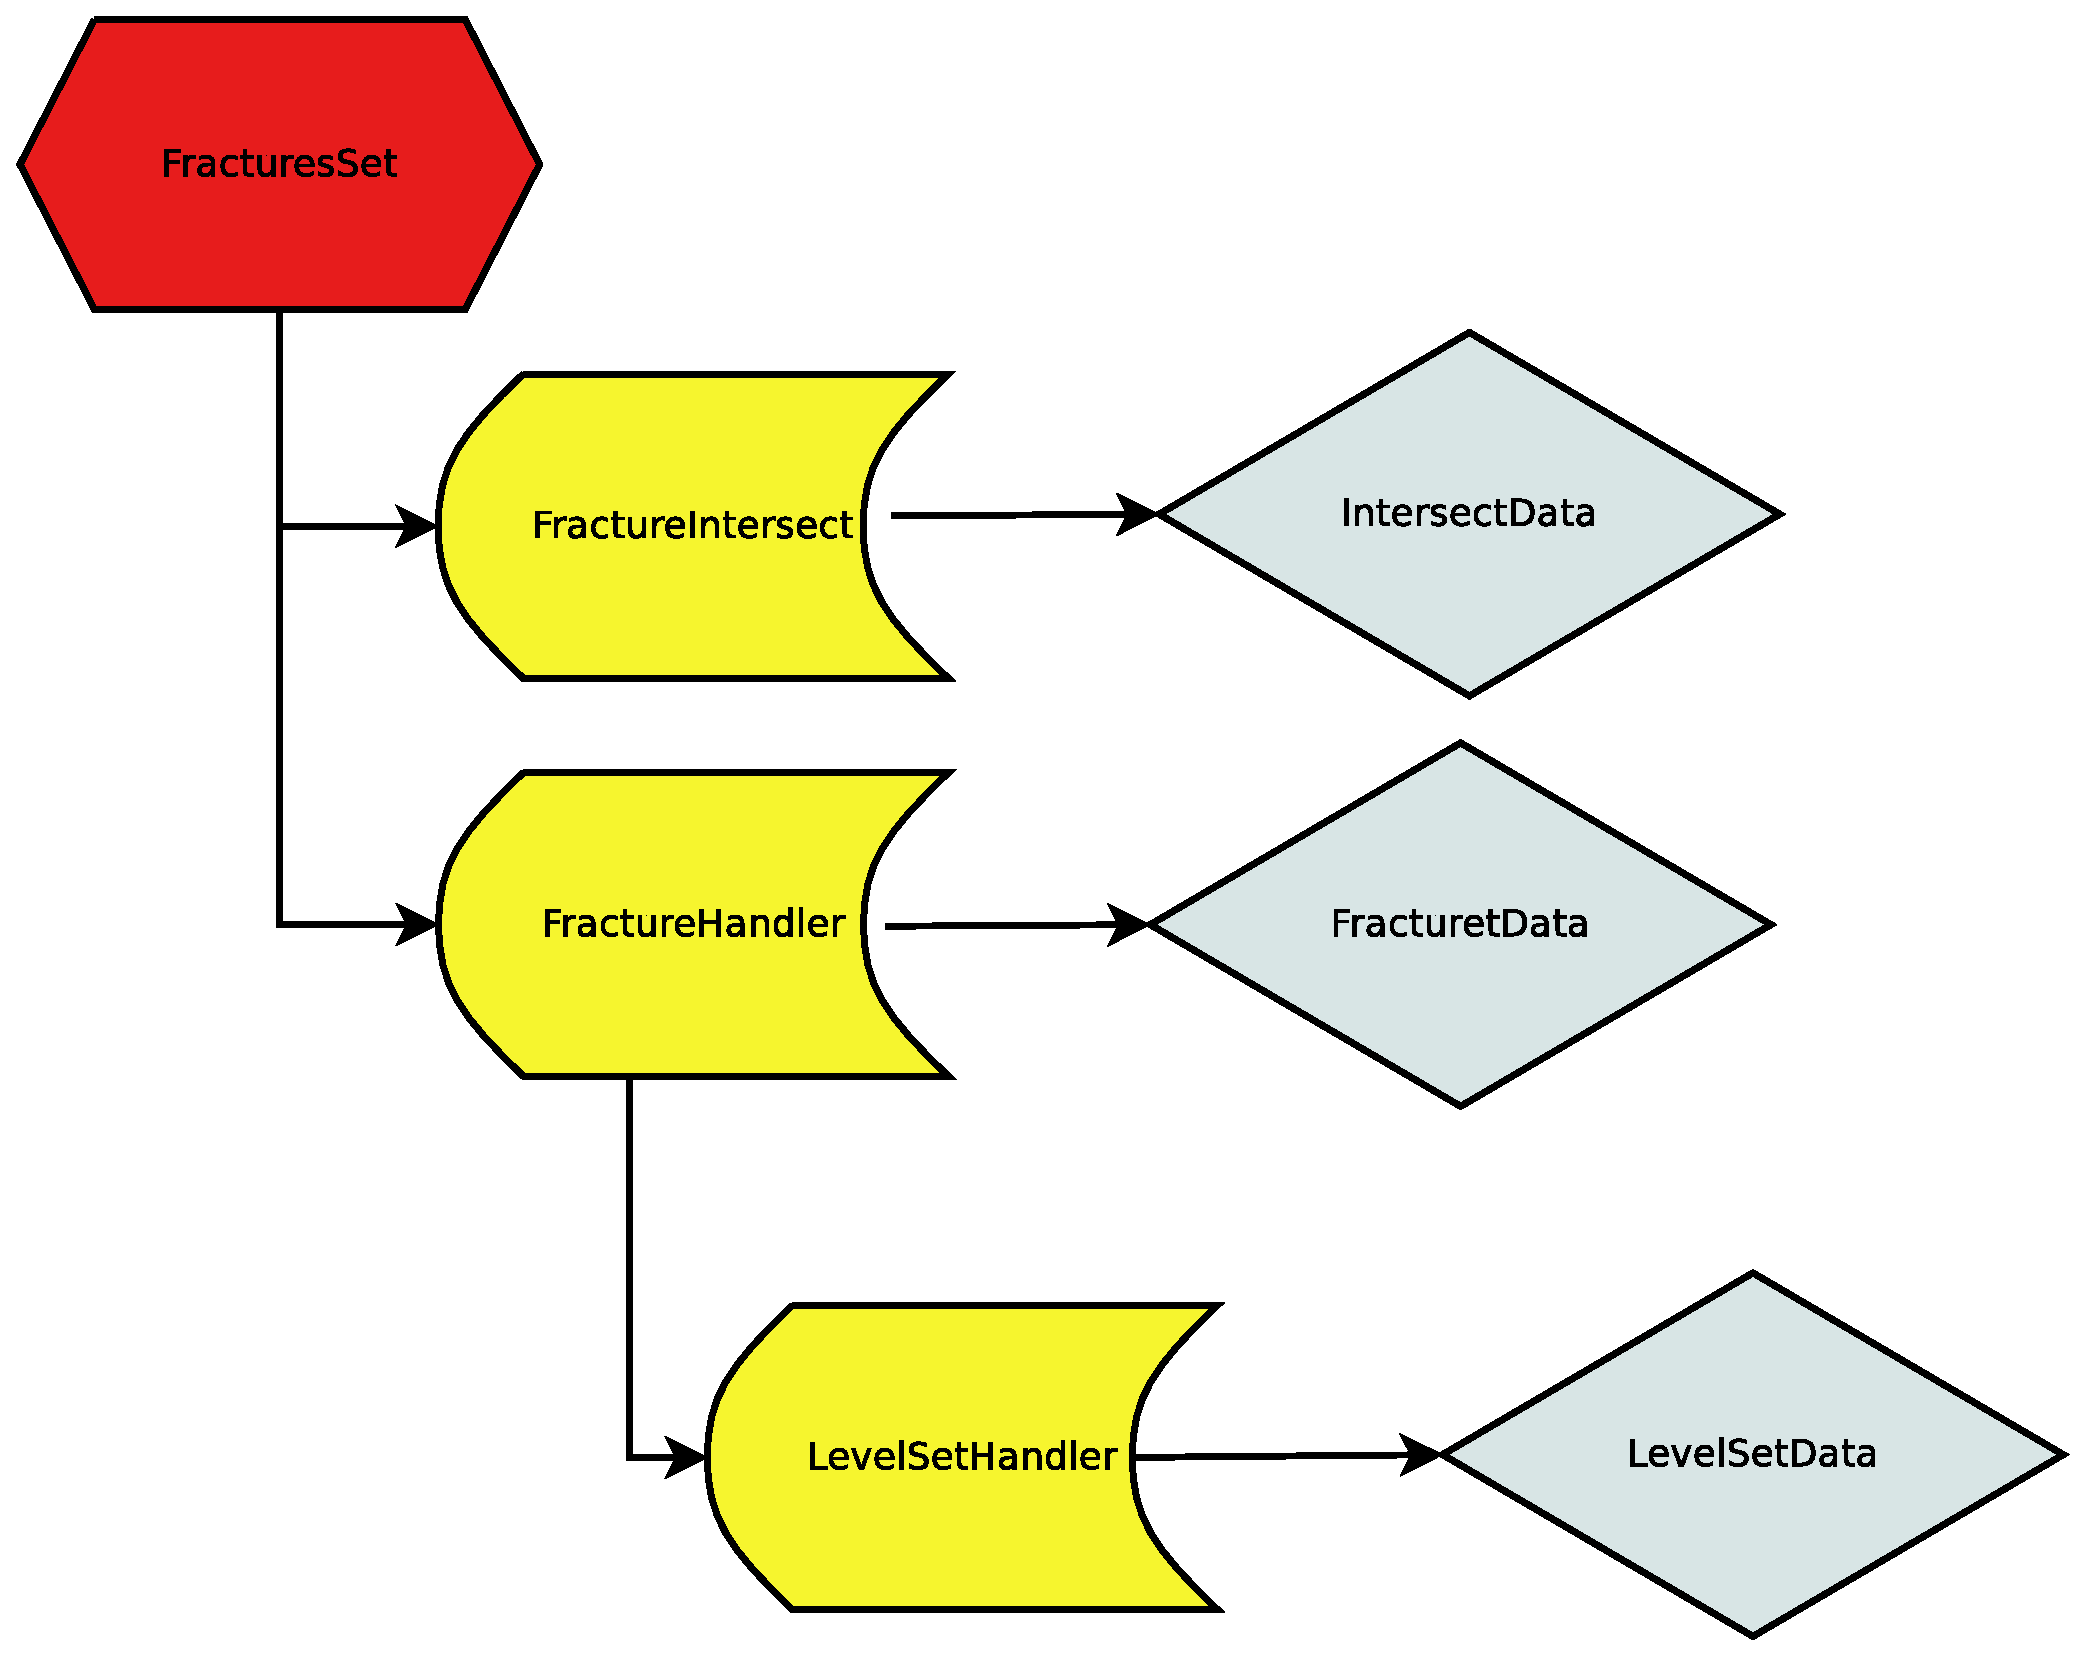
\includegraphics[width=1\textwidth]{img/fratture.eps}
\caption{Inclusione tra le varie classi che costituiscono l'insieme delle fratture}\label{Inclusione classi}
\end{figure}


\par Le classi usate per rappresentare le fratture e le intersezioni si dividono in due categorie:
\begin{enumerate}
\item[-] le classi in cui sono implementati tutti i metodi necessari per la costruzione e la manipolazione della grandezza ( insieme delle fratture, singola frattura, intersezioni, level set). Queste classi sono principalmente denominate col il suffisso \textit{Handler} e costituiscono l'ossatura dell'insieme delle fratture;
\item[-] le classi in cui sono contenuti tutti i parametri geometrici, fisici e le grandezze numeriche per l'implementazione e la risoluzione con elementi finiti, che riguardano la grandezza in esame. Vengono indicate con il suffisso \textit{Data} e rappresentano sempre un campo della corrispondente classe di tipo \textit{Handler}.
\end{enumerate}



\section{La Classe \texttt{FracturesSet}}
La class \texttt{FracturesSet} è la classe che contiente tutte le fratture e le rispettive intersezioni. La funzione che costruisce l'insieme delle fratture e le eventuali intersezioni è la funzione  \texttt{init}, che prende in input tutti i parametri necessari quali il numero di fratture, le mesh per l'integrazione e una variabile di tipo GetPot per la lettura dal file data. 

\begin{Code}[caption={Classe \texttt{FracturesSet}}]
class FracturesSet
{
public:

    enum
    {
        FRACTURE_UNCUT = 10000,
        FRACTURE_INTERSECT = 10000
    };

    FractureHandler ( const GetPot& dataFile,
                      const size_type& ID,
                      const std::string& section = "fractureData/" );

    void init ( );

    [ ... ]

private:
	FracturePtrContainer_Type M_fractures;

	FractureIntersectPtr_Type M_intersections;
	[ .... ]
};
\end{Code}
I campi principali della classe sono:
\begin{enumerate}
\item[-] \texttt{M\_fractures}, variabile di tipo vettore di puntatori alla classe \texttt{FractureHandler}  di cui parleremo più avanti, che rappresenta l'insieme di tutte le fratture;
\item[-] \texttt{M\_intersections}, un puntatore alla classe \texttt{FractureIntersect}, che rappresenta l'insieme di tutte le intersezioni. 
\end{enumerate}


\section{La Classe \texttt{FractureHandler}}

La classe  \texttt{FractureHandler} è la classe che inizializza e gestisce ogni frattura. I principali campi di questa classe sono:
\begin{enumerate}
\item[-] \texttt{M\_data}: classe \texttt{FractureData} che contiene tutte le informazioni circa la natura geometrica e fisica della singola frattura;
\item[-] \texttt{M\_levelSet}: puntatore alla classe \texttt{LevelSetHandler} di cui parleremo più avanti;
\item[-] i metodi di integrazione e le mesh per pressione e velocità;
\item[-] il vettore dei gradi di libertà estesi per velocità e pressione.
\end{enumerate}

La particolarità di questa classe è che possiede due mesh: una mesh 2d \texttt{M\_meshMapped} e una mesh 1d \texttt{M\_meshFlat}. Questo deriva dal fatto che le fratture sono su un piano e hanno una rappresentazione del tipo $y=f(x)$, cioè i loro punti hanno coordinate $(x,y)$. La libreria che noi usiamo, \textit{GetFEM++}, non è in grado di integrare su una mesh i cui punti hanno coordinate $(x,y)$ un'equazione 1d come quella del nostro modello ridotto. La tecnica è quindi quella di risolvere il problema integrando sulle mesh " piatte " 1d ottenute proiettando le mesh reali, e successivamente interpolare i risultati ottenuti per ritornare sulle mesh 2d. La creazione delle mesh è nella funzione \texttt{ init}.
\par La funzione principale di questa classe è  \texttt{setMeshLevelSetFracture }.
Tale funzione crea un legame tra la frattura corrente e le fratture con cui ha un'intersezione, tenendo traccia della mesh e dei valori del level set della frattura corrente nei punti della frattura intersecata. Nel caso di intersezione di tipo \textit{Cross}, dove l'intersezione tra due level set non è detto che avvenga su due punti delle rispettive mesh, vengono aggiunti i gradi di libertà estesi, due per la velocità e uno per la pressione. Nel caso dell'intersezione di tipo \textit{Bifurcation} l'introduzione di tali elementi non si rende necessaria.


\begin{Code}[caption={Funzione \texttt{setMeshLevelSetFracture}}]
size_type FractureHandler::setMeshLevelSetFracture ( 
					FractureHandler& otherFracture,
					size_type& globalIndex,
				         const std::string& type )
{	
[ ... ]
if ( !M_meshLevelSetIntersect[ otherFractureId ].get() )
{
   M_meshLevelSetIntersect[ otherFractureId ].reset
	 ( new GFMeshLevelSet_Type ( M_meshFlat ) );
   LevelSetHandlerPtr_Type otherLevelSet = otherFracture.getLevelSet();
   M_levelSetIntersect [ otherFractureId ].reset 
	( new GFLevelSet_Type ( M_meshFlat, 1, false )  );
   M_levelSetIntersect [ otherFractureId ]->reinit();

   const size_type nbDof = 
	M_levelSetIntersect [ otherFractureId ]->get_mesh_fem().nb_basic_dof();

   for ( size_type d = 0; d < nbDof; ++d )
   {
      base_node node = M_levelSetIntersect [ otherFractureId ]
			->get_mesh_fem().point_of_basic_dof(d);
      base_node mappedNode ( node.size() +1 );
      scalar_type t = d*1./(M_data.getSpatialDiscretization () );
      base_node P (node.size());
      P [0] = t;
      mappedNode [0] = node [0];
      mappedNode [1] = M_levelSet->getData()->y_map ( P );
      M_levelSetIntersect [ otherFractureId ]->values(0)[d] = 
	otherLevelSet->getData()->ylevelSetFunction ( mappedNode );
   }

   M_meshLevelSetIntersect[ otherFractureId ]
	->add_level_set ( *M_levelSetIntersect [ otherFractureId ] );
   M_meshLevelSetIntersect[ otherFractureId ]->adapt ();

   size_type i_cv = 0;
   dal::bit_vector bc_cv =
   M_meshLevelSetIntersect[ otherFractureId ]->linked_mesh().convex_index();
		
   for ( i_cv << bc_cv; i_cv != size_type(-1); i_cv << bc_cv )
   {
     if ( M_meshLevelSetIntersect[ otherFractureId ]->is_convex_cut ( i_cv ) )
     {  
        if ( type == "Cross")
        {	
           M_meshFlat.region ( FractureHandler::FRACTURE_UNCUT 
		* ( M_ID + 1 ) ).sup ( i_cv );
	 M_meshFlat.region ( FractureHandler::FRACTURE_INTERSECT 
		* ( M_ID + 1 ) + otherFractureId + 1 ).add( i_cv );
	 M_extendedPressure.push_back ( 
		M_meshFEMPressure.ind_basic_dof_of_element ( i_cv )[0] );
	 M_extendedVelocity.push_back ( 
		M_meshFEMVelocity.ind_basic_dof_of_element ( i_cv )[0] );
	 M_extendedVelocity.push_back ( 
		M_meshFEMVelocity.ind_basic_dof_of_element ( i_cv )[1] );
        }
            	
       M_fractureIntersectElements [ otherFractureId ].push_back ( i_cv );
	
           [ ... ]
      }
   }
}

return numIntersect;
}
\end{Code}


\section{Le Classi \texttt{LevelSetHandler} e \texttt{LevelSetData}}
Le fratture sono rappresentate come delle rette, funzioni $y=f(x)=ax+c$. Ad ogni frattura è associata una funzione level set  del tipo $f(x,y)=y-ax-b$ che divide il piano in due semipiani: i punti un cui $f(x,y)>0$ e i punti in cui $f(x,y)<0$. I punti in cui $f(x,y)=0$ sono quelli in cui è definita la frattura. 
\par La classe \texttt{LevelSetHandler} inizializza il levelset associato alla frattura. 
La funzione fondamentale della classe è la funzione \texttt{init}, funzione che inizializza il level set, definisce i metodi di integrazione e aggiunge alla mesh di supporto l'informazione legata al level set. I campi fondamentali della classe sono:
\begin{enumerate}
\item[-] \texttt{M\_data}: puntatore alla classe \texttt{LevelSetData}, classe che contiene tutte le informazioni sul level set e le funzioni per valutarne il valore nei punti;
\item[-] \texttt{M\_mesh}: puntatore ad una variabile di tipo \textit{getfem::mesh\_level\_set}, classe che contiene informazioni sulla mesh tagliata da level set;
\item[-] \texttt{M\_levelSet}: oggetto di tipo \textit{getfem::level\_set}, variabile che definisce il level set. In GetFEM un level set è rappresentato come una o due funzioni scalari, definito su una mesh di tipo \textit{getfem::mesh\_fem}, ossia una mesh su cui è definito un metodo ad elementi finiti.
\end{enumerate}

\begin{Code}[caption={Classe \texttt{LevelSetHandler}}]
class LevelSetHandler
{
public:

    LevelSetHandler ( const GetPot& dataFile, 
			const std::string& section =  "fractureData/", 
    			const std::string& sectionLevelSet = "levelSet/" );

    void init ( getfem::mesh& mediumMesh,
		    const std::string& mediumIntegrationTypeVelocity,
		    const getfem::mesh_fem& mediumMeshFEMPressure,
		    const getfem::mesh_fem& mediumMeshFEMVelocity );

	[ ... ]
private:

    LevelSetDataPtr_Type M_data;

    GFMeshLevelSetPtr_Type M_mesh;

    GFLevelSetPtr_Type M_levelSet;
	[ ... ]
};
\end{Code}


 \section{Le Classi \texttt{FractureIntersect} e \texttt{IntersectData}}

La classe \texttt{FractureIntersect} rappresenta tutte le intersezioni tra le fratture. Ad ogni tipo di intersezione viene associato il vettore delle classi \texttt{IntersectData}, classe che rappresenta la vera e propria intersezione, tenendo traccia delle informazioni sulle fratture e dell'id dell'elemento della mesh di supporto in cui avviene l'incontro.
\par Le intersezioni vengono classificate come \textit{Parallel}, \textit{Cross} e \textit{Bifurcation}.  L'idea alla base della classificazione è quella di considerare gli elementi della mesh 2d di supporto, la mesh del mezzo, in cui passano due o più fratture, e di associargli un flag:
\begin{enumerate}
\item[-] \textit{Parallel}: quando due o più fratture passano in uno stesso elemento della mesh ma non si intersecano;
\item[-] \textit{Cross}: quando due fratture passano nello stesso elemento della mesh e si intersecano formando una \textit{X};
\item[-] \textit{Bifurcation}: quando tre fratture si intersecano in un punto comune formando una \textit{Y}.
\end{enumerate}

\begin{Code}[caption={Funzione \texttt{constructIntesection}}]
void FractureIntersect::constructIntesection ( 
	const getfem::mesh& mesh, getfem::mesh_level_set& meshLevelSet, 
	const FracturePtrContainer_Type& fractures )
{
[ ... ]
meshLevelSet.find_level_set_potential_intersections ( 
			listOfConvex, listOfLevelSet_bitVector );

sizeVectorContainer_Type listOfLevelSet ( listOfConvex.size() );

if( listOfConvex.size() > 0 )
{
   for ( size_type i = 0 ; i < listOfConvex.size(); ++i )
   {
      // Conversione da un vettore di bit a un vettore di interi
      fromBitVectorToStdVector ( 
      listOfLevelSet_bitVector [ i ], listOfLevelSet [ i ] );

       // Per ogni elemento della mesh di supporto in cui passano 
      // almeno due fratture verifico il tipo di intersezione
       IntersectionType type = intersectionType ( 
		meshLevelSet, listOfConvex [ i ], listOfLevelSet [ i ] );
	        
       // Prendo i puntatori alle fratture coinvolte
      FracturePtrContainer_Type fracturesInvolved ( listOfLevelSet[i].size() );

      for ( size_type f = 0; f < fracturesInvolved.size(); ++f )
      {
	 fracturesInvolved [ f ] = fractures [ listOfLevelSet [ i ] [ f ] ];
       }
       // Costruisco la classe IntersectData per la nuova intersezione 
       // e la aggiungo in base al tipo
      IntersectData intersection;
      intersection.setIntersection ( listOfConvex[i], fracturesInvolved );		
      M_intersections [ type ].push_back ( intersection );
    }
[ ... ]
}

\end{Code}

\par La funzione  \texttt{constructIntesection} contiene la classificazione delle intersezioni. In questa funzione viene data una numerazione globale alle intersezioni, prima quelle di tipo \textit{Cross} e poi quelle di tipo  \textit{Bifurcation}.  Nel caso delle prime vengono aggiunte due nuove incognite, una per ogni frattura, necessarie per imporre le condizioni d'interfaccia nella formulazione debole del problema. Queste nuove variabili rappresentano la pressione nel punto di intersezione e  vengono poi accoppiate in modo da risultare uguali. Nel secondo caso invece si introduce una sola incognita per ogni intersezione, variabile che rappresenta la pressione nel punto d'incontro. Per ogni frattura coinvolta inoltre si tiene traccia del grado di libertà in cui avviene l'intersezione. Questo perchè, come vedremo, la condizione al contorno deve essere imposta solo del grado di libertà dell'estremo libero della frattura.

\section{Le Classi \texttt{BC} e \texttt{BCHandler}}
%\subsection{Definizione della classe e costruttore}
La classe \texttt{BC} ci permette di imporre le condizioni al bordo in ogni singola frattura. Per ogni frattura è necessario imporre due condizioni al contorno\\ 

%\newpage	
\begin{Code}[caption={Classe \texttt{BC}}]
class BC
{
 public:

    enum
    {
        DIRICHLET_BOUNDARY_NUM = 40,
        NEUMANN_BOUNDARY_NUM = 50
    };

    // Costruttore
    BC ( getfem::mesh& mesh,
         const std::string& MeshType,
         const sizeVector_Type DOFs,
         const ElementDimension& dimension = MEDIUM );

 private:

    getfem::mesh_fem M_meshFEM;
    
    sizeVector_Type M_dirichlet;
    sizeVector_Type M_neumann;
    sizeVector_Type M_extBoundary;   
};
\end{Code}

Quando si considera una frattura priva di intersezioni o con solo intersezioni di tipo \textit{Cross} le condizioni al contorno vengono imposte rispettivamente sul primo e l'ultimo gradi di libertà della mesh.\\
Nel caso della biforcazione, invece, bisogna accertarsi di imporre le condizioni al bordo solamente nell' estremo libero, ovvero quello in cui non sia presente alcuna intersezione. 
Per far questo motivo quando costruiamo l'insieme delle intersezioni per ogni frattura salviamo un vettore contenente l'indice dei gradi di libertà in cui c'è un'intersezione.

La classe \texttt{BCHandler} viene usata per gestire le condizioni al contorno sulle fratture.

\lstnewenvironment{Code03_03}[1][]{\lstset{basicstyle=\small\ttfamily, columns=fullflexible,framexrightmargin=+.1\textwidth, keywordstyle=\color{red}\bfseries, commentstyle=\color{blue},language=C++, basicstyle=\small, numbers=left, numberstyle=\tiny, stepnumber=1, numbersep=5pt, frame=shadowbox, #1}}{}

\chapter{Classi per la gestione dell'intersezione}

Nel modello che abbiamo preso in considerazione noi le fratture hanno una rappresentazione in $\mathbb{R}$ e, nel caso della \textit{Biforcazione}, hanno un unico punto in comune. 
Nella rappresentazione 2D, invece, la regione in comune è un triangolo. \\

\begin{figure}[htbp]
\centering
\includegraphics[scale=.5]{img/subcap3_3/TriangoloBiforcazione.eps}
%\includegraphics[width=0.65\textwidth]{img/TriangoloBiforcazione.eps}
\caption{Struttura della biforcazione 2D}\label{Biforcazione}
\end{figure}

Il nostro modello trascura ovviamente delle informazioni, ma nel caso di fratture con uno spessore sufficientemente piccolo rispetto a quelle del dominio, può essere considerato una buona approssimazione della realtà.\\

Per ricavare le condizioni d'interfaccia nel caso della biforcazione per modello ridotto passiamo per la rappresentazione in $\mathbb{R}^{2}$.
Nel caso 2D le fratture hanno uno spessore e possiamo delimitare un triangolo di intersezione unendo i punti di incontro dei loro bordi. \\
Presi \textbf{N} il vettore delle normali ai lati del triangolo, \textbf{$K_{I}$} la matrice di permeabilit\`{a} all'intersezione e una costante \textit{t} possiamo definire:
\begin{center}
	$ S = \textit{t} \, diag( \textbf{N}$ \textbf{$K_{I}$} $ \textbf{N}^{T} ) $
\end{center}
Definite ora \textbf{C} matrice dei vettori che uniscono il baricentro, punto C, del triangolo con il punto medio  di ogni lato e \textbf{$P_{c}$} matrice di proiezione sullo spazio nullo della matrice di base per \textbf{C}, possiamo trovare la matrice di trasmissibilit\`{a}:
\begin{center}
	$ T = \frac{1}{\textbf{I}}( \textbf{N}$ \textbf{$K_{I}$} $ \textbf{N}^{T} ) + $\textbf{$P_{c}$} $\textbf{S}$\textbf{$P_{c}$}
\end{center}
%\textbf{u} = \left\lbrace \u_{0}, \u_{1}, \u_{2} \right\rbrace
%$\textbf{\pi} = \left\lbrace \pi_{0}, \pi_{1}, \pi_{2} \right\rbrace $
Le variabili con cui ci troviamo a lavorare sono:
	\begin{enumerate}
	\item[-] \textbf{u} : vettore dei flussi
	\item[-] $p_{I}$ :  pressione nel punto di intersezione delle assi delle tre fratture;
	\item[-] \textbf{$\pi$}: vettore delle pressioni nel punto di incontro fra l'asse della frattura i-esima con un lato del triangolo;
	\end{enumerate} 
e le condizioni che dobbiamo porre all'intersezione sono:
\begin{center}			
	$\left \{
		\begin{array}{l}	
	 		\textbf{u} - p_{I}T\textbf{1}_{3}+T \boldsymbol{\Pi}=0  \\ \\
     	 	\displaystyle \sum_{k=0}^2 u_{k} = p_{I} - \pi  \\
		\end{array}
	\right.$
\end{center} \label{condizioni d'interfaccia}

\noindent  Queste sono le condizioni d'interfaccia che verranno imposte nel punto di intersezione delle fratture.\\ 
\par In questa parte di codice per gestire sia il calcolo delle matrici introdotte precedentemente, che i punti e la geometria del triangolo di intersezione, abbiamo usato la libreria matematica \textit{Eigen}.\\
\par Note le basi teoriche possiamo passare a descrivere le principali classi del codice che definiscono la struttura e le propriet\`{a} della biforcazione in uno spazio bidimensionale.

\newpage
\begin{figure}[htbp]
\centering
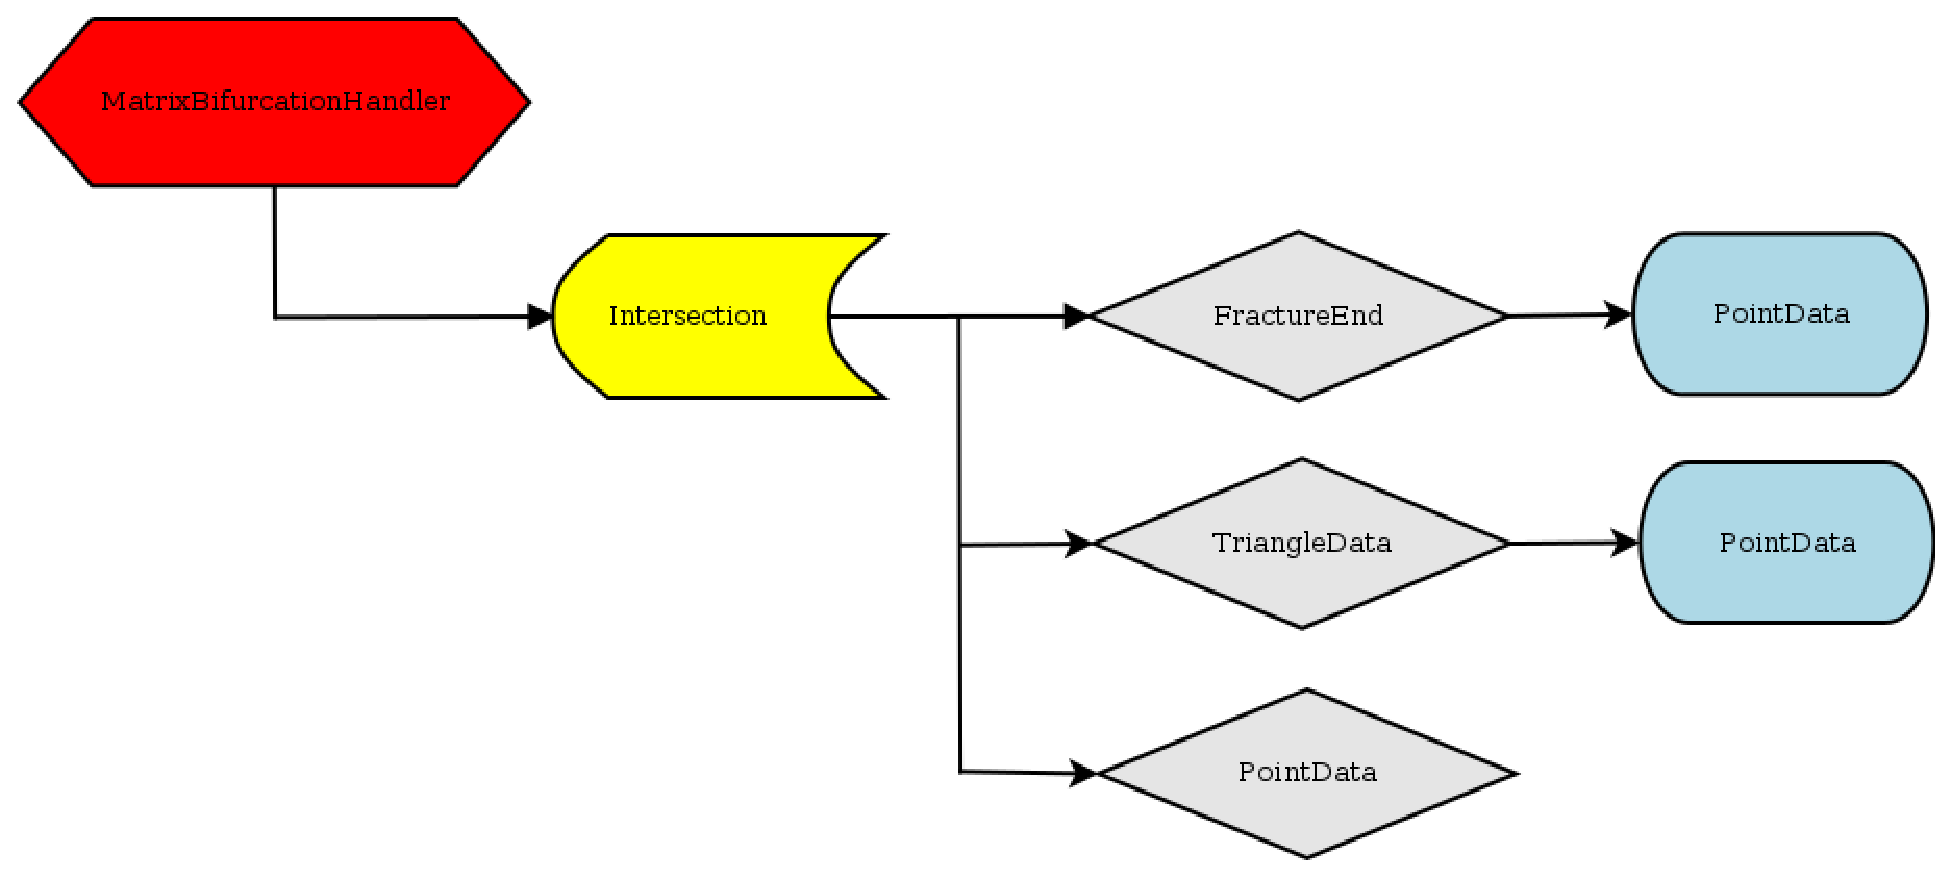
\includegraphics[height=7cm, width=1\textwidth]{img/subcap3_3/MatrixBifurcationHandler2.eps}
\caption{Inclusione tra le varie classi che costituiscono il triangolo di intersezione}\label{Inclusione classi MatrixBifurcationHandler}
\end{figure}

\section{La Classe \texttt{MatrixBifurcationHandler}}
La classe \texttt{MatrixBifurcationHandler} contiene le matrici associate a una biforcazione e implementa i metodi per calcolarle.  Il fine ultimo è il calcolo della matrice di trasmissibilità T.

\noindent I campi fondamentali della classe sono:
	\begin{enumerate}
	\item[-] \texttt{M\_intersection}: di tipo Intersection, contiene tutte le informazioni base per poter ricavare le matrici;
	\item[-] \texttt{M\_T}: matrice T di trasmissibilità necessaria per l'imposizione delle condizioni di interfaccia.
	\end{enumerate} 
\begin{Code03_03}[caption={Classe \texttt{Intersection}}]
class MatrixBifurcationHandler
{
 public:
	MatrixBifurcationHandler( const GetPot& dataFile,
				const std::string& section = "mediumData/",
				const std::string& subsection = "darcy/");
	
	void setMatrices ( FracturePtrContainer_Type& fractures );
	
	[ ... ]
	
	void computeT( scalar_type t=6.0 );

	[ ... ]

 private:

	Matrix2d M_K;
	Intersection_Type M_intersection;
	Matrix32 M_N;
	Matrix32 M_C;
	Matrix32 M_Qc;
	Matrix3d M_Pc;
	Matrix3d M_T;
};
\end{Code03_03}

\section{La Classe \texttt{Intersection}}

La class \texttt{Intersection}, definita in \texttt{Geometry.h}, contiene tutte le informazioni relative ad una biforcazione in uno spazio 2D necessarie per il calcolo delle matrici associate al triangolo di intersezione.
I campi fondamentali della classe sono:
	\begin{enumerate}
	\item[-] \texttt{M\_intersection}: di tipo PointData, rappresenta il punto di intersezione;
	\item[-] \texttt{M\_tangents}: vettore contenente le tangenti alle fratture coinvolte;
	\item[-] \texttt{M\_normals}: vettore contenente le normali alle fratture coinvolte;
	\item[-] \texttt{M\_intersectionTriangle}:di tipo TriangleData, rappresenta il triangolo di intersezione, i cui vertici sono i punti d'incontro dei bordi delle fratture.
	\end{enumerate} 

\begin{Code03_03}[caption={Classe \texttt{Intersection}}]
class Intersection
{
 public:
	[ ... ]
	
	void setIntersection( FracturePtrContainer_Type& M_FracturesSet );
	
	[ ... ]
 private:
	
	[ ... ]	
	
	PointData M_intersection;
	
	Vector2d M_tangents [ 3 ];
	Vector2d M_normals [ 3 ];
	
	TriangleData M_intersectionTriangle;
};	
\end{Code03_03}

\section{Classe \texttt{PointData} e Classe \texttt{TriangleData}}
Queste classi rappresentano un punto e un triangolo come grandezze geometriche.
Il punto geometricamente viene rappresentato come una grandezza zero dimensionale con due variabili, una \textit{x} e una \textit{y}.
Un triangolo è invece  rappresentato geometricamente dai punti che lo costituiscono.\\
\noindent La classe \texttt{PointData} ci permette di definire un punto e di poterlo manipolare con le operazioni di somma, differenza e prodotto.\\
\noindent La classe \texttt{TriangleData} ci permette di definire un triangolo e di calcolarne l'area. Inoltre sono stati implementati i metodi necessari per la costruzione del triangolo di intersezione.


\section{Normativa di riferimento}
La giurisprudenza italiana negli ultimi anni si \`e dotata di un
complesso di norme volte a guidare le aziende nel raggiungimento di un
equilibrio tra quanto le tecnologie consentono di realizzare e la
necessit\`a di proteggere dati che spesso non appartengono ai singoli
soggetti che li gestiscono. Adempiere alla normativa in materia di
sicurezza delle informazioni significa, quindi, evitare il rischio
legale ovvero di incorrere in sanzioni penali/amministrative a seguito
del mancato adempimento di leggi o regolamenti. Di seguito sono
brevemente riportate le normative che hanno impatti
sull'I\&AM.

\subsection{Codice in materia di protezione dei dati personali}

Il nuovo Codice in materia di protezione dei dati personali (D.lgs.
196/03), entrato in vigore dal primo gennaio 2004, disciplina alcuni
aspetti relativi all'identity \& Access Management.
Alla base delle nuove misure minime sono infatti poste le modalit\`a
per l'accesso ai dati, che devono avvenire solo da
parte di persone autorizzate ed esplicitamente incaricate; a esse
dovranno essere assegnate o associate credenziali di
autenticazione che dovranno consentire
l'autenticazione delle persone incaricate al
trattamento dei dati. Inoltre quando pi\`u incaricati accedono ai dati
\`e necessario associare a ogni soggetto uno specifico profilo di
accesso. Il profilo identifica i trattamenti di dati che possono essere
svolti e costituisce l'ambito del trattamento
consentito.

Di seguito sono riportate in dettaglio le misure minime che impattano
sui processi di I\&AM.


\textbf{Procedura di autenticazione} (rif. Punto 1, Disciplinare Tecnico)

Il singolo strumento elettronico utilizzato all'interno
di un trattamento di dati personali deve prevedere una procedura di
autenticazione


\textbf{Formato delle credenziali di autenticazione} (rif. Punto 2, Disciplinare Tecnico)

Le credenziali di autenticazione devono essere costituite da un codice
per l'identificazione dell'incaricato associato ad una parola chiave oppure da un dispositivo di
autenticazione eventualmente associato ad un codice identificativo o ad
una parola chiave, ovvero da una caratteristica biometrica.


\textbf{Associazione tra codici di identificazione (login) e incaricati} (rif. Punto 3, Disciplinare Tecnico)

Ogni incaricato pu\`o avere pi\`u credenziali di autenticazione (pi\`u
login), tuttavia la singola credenziale deve essere associata e
riconducibile ad un singolo utente (non \`e permessa quindi la
condivisione della conoscenza di credenziali di autenticazione)


\textbf{Norme per l'uso delle password} (rif. Punto 4, Disciplinare Tecnico)

Devono essere definite e diffuse norme per il mantenimento della
segretezza delle password nel tempo (le password non devono essere
annotate in prossimit\`a della postazione di lavoro, non devono essere
comunicate a terzi, \ldots).


\textbf{Lunghezza minima della password} (rif. Punto 5, Disciplinare tecnico)

La password deve essere lunga almeno 8 caratteri (laddove non sia
possibile la lunghezza massima consentita).


\textbf{Formato della password} (rif. Punto 5, Disciplinare tecnico)

La password deve essere composta da caratteri alfanumerici, non banale
(non consistere in parole di senso compiuto) e non deve contenere
riferimenti agevolmente riconducibili all'incaricato.


\textbf{Cambio Password Obbligatorio al primo utilizzo} (rif. Punto 5, Disciplinare tecnico)

La password deve essere modificata dall'utente dopo il primo accesso.


\textbf{Autonoma sostituzione della password} (rif. Punto 5, Disciplinare tecnico)

Per garantire la segretezza della password, l'utente
deve essere in grado di effettuare un'autonoma
sostituzione della password.


\textbf{Cambio Password Periodico} (rif. Punto 5, Disciplinare tecnico)

La password deve essere modificata almeno ogni 6 mesi (3 mesi nel caso
di trattamento dati sensibili).


\textbf{Non riutilizzo dei codici di identificazione} (rif. Punto 6, Disciplinare tecnico)

Nel caso in cui un incaricato (un utente) perda le qualit\`a per
accedere ai dati coinvolti nel trattamento, la sua corrispondente
utenza (le sue credenziali) non va cancellata ma disabilitata: questo
\`e fondamentale affinch\'e la stessa login non possa essere assegnata,
anche in tempi futuri, ad un'altra persona.


\textbf{Procedure formali per la gestione delle utenze} (rif. Punto 3,7,8, Disciplinare tecnico)

Devono esistere procedure per la gestione del ciclo di vita delle utenze
(creazione, disabilitazione temporanea, disabilitazione definitiva,
modifica del profilo di autorizzazione)


\textbf{Revoca per inutilizzo} (rif. Punto 7, Disciplinare tecnico)

L'utenza che non accede al sistema per un periodo
superiore a 6 mesi deve essere disattivata (la sua abilitazione deve
richiedere l'intervento di un amministratore).


\textbf{Disattivazione delle credenziali in caso di perdita delle qualit\`a}
(rif. Punto 8, Disciplinare tecnico)

Deve essere prevista una procedura che assicuri, nel caso in cui un
incaricato (un utente) perda le qualit\`a per accedere ai dati
coinvolti nel trattamento, che la sua corrispondente utenza (le sue
credenziali) venga disabilitata (non cancellata).


\textbf{Revisione Annuale dei profili di autorizzazione} (rif. Punto 14,
Disciplinare tecnico)

Deve essere redatta una procedura per la revisione almeno annuale della
sussistenza delle condizioni per la conservazione dei profili di
autorizzazione.


\textbf{Elenco degli incaricati e dei profili di autorizzazione}
(rif. Punto 15, Disciplinare tecnico)

Nell'ambito della revisione annuale dei profili di
autorizzazione \`e necessario redigere per iscritto la lista degli
incaricati, anche per classi omogenee, e dei relativi profili di
autorizzazione


\subsection{Illeciti amministrativi, D.lgs. 231}

Con l'emissione del Decreto Legislativo 231 dell'8 Giugno 2001, l'Italia ha
recepito la normativa europea relativa alla lotta contro la corruzione ed ha
disciplinato la responsabilit\`a amministrativa delle persone giuridiche e degli
enti privi di personalit\`a giuridica nel caso dei reati commessi dal vertice
aziendale o dai propri dipendenti/collaboratori sottoposti alla vigilanza del
vertice.

Oggetto della responsabilit\`a sono i reati contro la Pubblica Amministrazione
(corruzione, concussione, malversazione, frode, truffa, indebita percezione di
erogazioni), nonch\'e i reati cd. societari (false comunicazioni sociali, falso
in prospetto, impedito controllo, formazione fittizia del capitale, indebita
restituzione dei conferimenti, illegale ripartizione degli utili e delle
riserve, infedelt\`a patrimoniale).

L'adozione di un modello di IAM, \`e uno degli elementi che consentono di
recepire ed integrare nelle procedure aziendali la normativa relativa alla
introduzione nell'ordinamento nazionale del principio di responsabilit\`a
amministrativa degli enti e di progettare ed efficacemente attuare il sistema di
prevenzione e di auditing dinamico idoneo a ridurre il rischio di commissione
dei reati contemplati dal DLgs 231, anche in prospettiva
dell'evoluzione normativa e di probabile estensione dei principi del Decreto ad
altri ambiti (reati ambientali, reati commessi in violazione delle norme sulla
sicurezza sul lavoro).

\section{Analisi del modello organizzativo}

\subsection{Funzioni aziendali coinvolte nei processi di Identity and Access Management}

Di seguito sono elencate le funzioni aziendali coinvolte nei processi di
gestione degli utenti e delle relative credenziali e per ogni funzione
coinvolta sono descritte le principali attivit\`a in ambito IAM.
Le mansioni indicate sono relative all'azienda presso cui ho effettuato lo
stage.

%\begin{table}
%\begin{tabular}{|l||l|}
%\hline
%\textbf{Funzione Aziendale} & \textbf{Ruolo nei processi di Identity e Access Management} \\
%%\endhead
%\hline
%
%Funzioni principali & \\
%\hline
%
%\textbf{Settore Risorse Umane} & 
%\textbullet Richiesta aggiornamento utenze personale dipendente in 
%seguito ad assunzione, trasferimento, distacco o dimissioni.
%\textbullet Registrazione delle informazioni anagrafiche e di inquadramento 
%nella struttura organizzativa dei dipendenti nel DB
%\\
%\hline
%
%\textbf{Responsabili Uffici della Societ\`{a}} & 
%\textbullet Definizione dei livelli di accesso alle applicazioni 
%di propria competenza 
%\textbullet Compilazione richiesta aggiornamento utenze per le applicazioni 
%che non rientrano nello standard dell'unit\`{a} organizzativa
%\textbullet Compilazione richiesta abilitazione utenze esterne
%\\
%\hline
%
%\textbf{Ufficio Sistemi Operativi e Network Nucleo Gestione Operativa} & 
%\textbullet Aggiornamento delle utenze nei sistemi informatici aziendali, 
%sulla base degli schemi standard dei profili utenti previsti 
%per le unit\`{a} organizzative aziendali, e/o delle specifiche 
%richieste effettuate attraverso il workflow di Richieste HW e SW o tramite mail. 
%Tale attivit\`{a} viene svolta, ove necessario, coordinandosi con 
%gli uffici Sviluppi Applicativi e Progetto Piattaforma Virtuale 
%e Knowledge Management.
%\textbullet Comunicazione attivazione/ variazione/ disattivazione 
%utenza tramite workflow ``Gestione Utenze di Sistema'' al Nucleo 
%Sicurezza Informatica.
%\textbullet Registrazione delle informazioni anagrafiche relative 
%agli utenti esterni.
%\\
%\hline
%
%\textbf{Nucleo Compliance, Privacy e Sicurezza Informatica} & 
%\textbullet Definizione delle policy di sicurezza informatica 
%\textbullet Ricezione, nella ToDo list dell'Area Operativa, delle comunicazioni di avvenuto aggiornamento delle utenze nei sistemi aziendali. 
%\textbullet Aggiornamento database generale delle utenze aziendali 
%\textbullet Monitoraggio della situazione dei profili utente nei sistemi informatici
%aziendali, al fine di verificare la corretta gestione dei dati trattati e della
%loro sicurezza (come previsto dalla normativa sulla privacy (D.lgs. 196/2003).
%Sono verificati in particolare il corretto aggiornamento dei profili dimessi e
%l'adeguatezza dei parametri censiti per ogni utente rispetto allo standard
%previsto per l'unit\`{a} aziendale di appartenenza.  
%\\
%\hline
%
%\textbf{Responsabile Area IT} & 
%\textbullet Definizione, in collaborazione con i responsabili degli 
%uffici della dotazione standard delle unit\`{a} organizzative.
%\\
%\hline
%
%\textbf{Funzioni ausiliarie} &
%\\
%\hline
%
%\textbf{Organizzazione} & 
%\textbullet Formalizzazione delle procedure di I\&AM
%\\
%\hline
%
%\end{tabular}
%\end{table}
\begin{sidewaystable}
\begin{tabular}{|p{10cm}||p{10cm}|}
\hline 
\textbf{Funzione Aziendale}  & \textbf{Ruolo nei processi di Identity e Access Management} \tabularnewline
\hline 
%\endhead
%Funzioni principali  & \tabularnewline
%\hline 
\textbf{Settore Risorse Umane}  & \textbullet Richiesta aggiornamento utenze personale dipendente in
seguito ad assunzione, trasferimento, distacco o dimissioni. 
\textbullet Registrazione delle informazioni anagrafiche e di inquadramento nella
struttura organizzativa dei dipendenti nel DB \tabularnewline
\hline 
\textbf{Responsabili Uffici della Società}  & \parbox[t]{10cm}{\textbullet Definizione dei livelli di accesso alle applicazioni
di propria competenza \\
\textbullet Compilazione richiesta aggiornamento utenze per le applicazioni
che non rientrano nello standard dell'unità organizzativa\\
\textbullet Compilazione richiesta abilitazione utenze esterne }\tabularnewline
\hline 
\textbf{Ufficio Sistemi Operativi e Network Nucleo Gestione Operativa}  & \parbox[t]{10cm}{\textbullet Aggiornamento delle utenze nei sistemi informatici aziendali,
sulla base degli schemi standard dei profili utenti previsti per le
unità organizzative aziendali, e/o delle specifiche richieste effettuate
attraverso il workflow di Richieste HW e SW o tramite mail. Tale attività
viene svolta, ove necessario, coordinandosi con gli uffici Sviluppi
Applicativi e Progetto Piattaforma Virtuale e Knowledge Management.
\\
\textbullet Comunicazione attivazione/ variazione/ disattivazione
utenza tramite workflow ``Gestione Utenze di Sistema'' al Nucleo
Sicurezza Informatica.\\
\textbullet Registrazione delle informazioni anagrafiche relative
agli utenti esterni. }\tabularnewline
\hline 
\textbf{Nucleo Compliance, Privacy e Sicurezza Informatica}  & \parbox[t]{10cm}{
\textbullet Definizione delle policy di sicurezza informatica\\
\textbullet Ricezione, nella ToDo list dell'Area Operativa, delle comunicazioni
di avvenuto aggiornamento delle utenze nei sistemi aziendali. \\
\textbullet Aggiornamento database generale delle utenze aziendali
\textbullet Monitoraggio della situazione dei profili utente nei
sistemi informatici aziendali, al fine di verificare la corretta gestione
dei dati trattati e della loro sicurezza. 
%Sono verificati in particolare il
%corretto aggiornamento dei profili dimessi e l'adeguatezza dei parametri
%censiti per ogni utente rispetto allo standard previsto per l'unità
%aziendale di appartenenza.
}\tabularnewline
\hline 
\textbf{Responsabile Area IT}  & \textbullet Definizione, in collaborazione con i responsabili degli
uffici della dotazione standard delle unità organizzative. \tabularnewline
\hline 
%\textbf{Funzioni ausiliarie}  & \tabularnewline
%\hline 
\textbf{Organizzazione}  & \textbullet Formalizzazione delle procedure di I\&AM \tabularnewline
\hline
\end{tabular}
\caption{Ruoli e competenze}
\end{sidewaystable}


\subsection{Definizione e gestione dei profili di accesso}

I diritti di accesso ai sistemi informativi sono assegnati ad ogni
utente, in maniera incrementale, sulla base
dell'unit\`a organizzativa/ufficio di appartenenza e
del ruolo rivestito. Questo garantisce l'accesso ad un
insieme minimo di risorse informatiche collegate alle attivit\`a
lavorative dell'ufficio di appartenenza.
L'elenco delle risorse informatiche associate ad un
ufficio/nucleo costituiscono il profilo standard dello stesso.

Per garantire che tutti gli utenti abbiano accesso alle risorse
informatiche necessarie per il corretto svolgimento
dell'operativit\`a quotidiana, i diretti responsabili
possono chiedere abilitazioni aggiuntive ``ad personam''.

Le attribuzioni ad ``personam'' di
norma trovano applicazione solo fino a quando non cambia la
destinazione di un utente (ufficio); al cambiamento di questa ultima
infatti vengono eliminate tutte le abilitazioni
dell'ufficio di provenienza che non trovano
corrispondenza con l'ufficio di destinazione.

In generale, i profili di accesso (insieme dei diritti di accesso di un
utente) sono definiti dall'area IT su indicazione dei
Responsabili di Settore/Area che valutano la necessit\`a da parte del
richiedente del diritto di accesso sulla base delle attivit\`a
lavorative della struttura organizzativa del richiedente. 

I profili di accesso definiti vengono successivamente implementati
dall'area IT e controllati dal nucleo Sicurezza
Informatica. L'ufficio di Audit riveste il ruolo di
supervisore, per garantire che i ruoli assegnati siano i minimi
necessari allo svolgimento dell'attivit\`a lavorativa.


\subsection{Processi di I\&AM}

Di seguito sono riportati in forma sintetica i principali processi
connessi con la gestione del ciclo di vita delle utenze evidenziando le
funzioni aziendali coinvolte e gli strumenti utilizzati.

\subsubsection{Workflow creazione utenti interni (dipendenti, stagisti,
interinali)}


\textbf{Funzioni aziendali coinvolte}:Settore Risorse Umane,
Responsabili Uffici della Societ\`a, Nucleo Gestione Operativa, Nucleo Sicurezza
Informatica

Al momento dell'assunzione di un nuovo
dipendente/stagista, un responsabile del settore Risorse Umane
inserisce, attraverso il workflow \textit{Gestione Risorse Umane}
(\textit{Prevista Nuova Assunzione}), le informazioni anagrafiche e di
inquadramento nella struttura organizzativa che lo riguardano. In
particolare vengono inserite le seguenti informazioni:

\begin{itemize}
\item Informazioni anagrafiche proprie
dell'utente (Cognome e Nome, Nazionalit\`a, Data e
Indirizzo di nascita, Indirizzo di residenza, Data di Assunzione )
\item Informazioni di identificazione univoca (Codice Fiscale)
\item Informazioni di inquadramento nella struttura
Organizzativa (Societ\`a di appartenenza, Area, Struttura, Ufficio,
Nucleo, Tipi responsabilit\`a, Centro di Costo,\dots)
\end{itemize}

Il workflow ``Prevista nuova assunzione''
innesca il processo di assegnazione delle risorse (informatiche e fisiche)
all'utente;
vengono create le schede di lavoro e vengono inviate le notifiche via
mail al personale preposto alla gestione delle applicazioni
informatiche e alla gestione delle risorse fisiche (scrivanie,
telefono, macchine, \dots) e al nucleo Sicurezza Informatica. La
creazione delle utenze viene gestita dal Nucleo Gestione Operativa
attraverso il workflow \textit{Gestione Utenze di Sistema}. Dopo che
le utenze sono state create il nucleo Gestione Operativa inserisce
attraverso il workflow Gestione Risorse Umane le seguenti informazioni:

\begin{itemize}
\item Numero di telefono 
\item Indirizzo di e-mail
\end{itemize}

I profili di accesso sono attribuiti in base all'ufficio
o nucleo di appartenenza e al ruolo (responsabile od operatore).

Il giorno dell'assunzione (primo giorno effettivo di
lavoro del dipendente) viene inserita la matricola
dell'utente e viene chiuso il processo di registrazione
del nuovo dipendente. A questo punto l'utente viene
pubblicato nell'organico aziendale
all'interno dell'organigramma
visualizzabile attraverso il portale interno, e le sue utenze vengono
abilitate.

Per gli stagisti il processo \`e analogo a quello descritto per i
dipendenti. Per questi per\`o non esiste un profilo standard basato
sull'unit\`a organizzativa di appartenenza ma le
abilitazioni vengono gestite ``ad
personam'' su richiesta del tutore/responsabile
aziendale attraverso il workflow Richieste HW e SW e tramite e-mail.


\subsubsection{Workflow creazione utenti esterni (consulenti)}

\textit{Funzioni aziendali coinvolte}:Responsabili
Uffici della Societ\`a, Nucleo Gestione Operativa, Nucleo Sicurezza
Informatica


Non esistono profili di accesso standard per gli utenti esterni.
L'assegnazione delle credenziali di accesso agli utenti
esterni \`e gestita ``ad personam''
tramite una richiesta esplicita da parte del Responsabile/Tutor
aziendale del consulente (es. Project Leader). E'
quindi compito del responsabile del nuovo consulente, effettuare, prima
che quest'ultimo inizi a lavorare, una richiesta con
l'elenco delle risorse informatiche di cui il
consulente necessita per lavorare, tramite mail.

Ricevuta la notifica, l'unit\`a Gestione Operativa
registra il consulente all'interno del database
preposto, inserendo nome e cognome del consulente, societ\`a di
appartenenza e le applicazioni a cui l'utente pu\`o
accedere e crea le utenze richieste dal Responsabile
dell'utente. 

Gli utenti esterni vengono ulteriormente divisi in due gruppi:

\begin{itemize}
\item utenti in: sono i consulenti che svolgono
un'attivit\`a continuativa interna (es. application
management);
\item utenti out: sono i consulenti occasionali
\end{itemize}
Entrambe le tipologie di utenti sono censite, ma soltanto le utenze in a
cui generalmente deve essere associato un numero di telefono interno
vengono pubblicati sulla rubrica telefonica.


\subsubsection{Workflow rimozione utenti interni (dipendenti, stagisti)}


\textbf{Funzioni aziendali coinvolte}:Settore
Risorse Umane, responsabili Uffici della Societ\`a,
Nucleo Gestione Operativa, Nucleo Sicurezza Informatica


Quando un dipendente cessa un rapporto di collaborazione,
l'ufficio Risorse Umane inserisce la data prevista di
dimissioni in un apposito campo del record dell'utente
sul data base. 

Un processo notturno di gestione delle sospensioni si occupa di
disabilitare le utenze scadute, mantenendo tutti i dati relativi per 30
giorni, dopo di che vengono cancellate definitivamente.

L'ultimo giorno di lavoro del dipendente il sistema di
IAM completa il processo di rimozione utente eliminandolo
dall'organico, dal portale interno e dalla rubrica.

Nota: Rimane traccia di tutti gli utenti rimossi nel download
dell'applicativo Gestione Risorse Umane (export batch
in formato excel .csv dei dati anagrafici del personale in organico e
dimesso).

Per gli stagisti il processo di rimozione \`e analogo a quello del
dipendente ed \`e innescato dall'ufficio Risorse Umane.



\subsubsection[Workflow rimozione consulenti]{Workflow rimozione consulenti}

\textbf{Funzioni aziendali coinvolte}:Responsabili
Uffici della Societ\`a, Nucleo Gestione Operativa, Nucleo Sicurezza
Informatica


Data l'importanza che le credenziali di accesso
ricoprono ai fini della protezione dei dati aziendali, \`e necessario
prevedere la disabilitazione delle stesse in caso di mancato utilizzo e
a fronte di eventi che possano comprometterne la sicurezza (es.
cessazione rapporto di collaborazione o assenza prolungata).

Le policy aziendali prevedono che un account di un consulente abbia
durata pari a 4 mesi.
Dieci giorni prima della disabilitazione dell'account,
il nucleo Gestione Operativa invia una mail al responsabile del
consulente per verificare la necessit\`a di mantenere tale userid
ancora attiva.

In caso di risposta negativa il nucleo Gestione Operativa disabilita e
dopo 30 giorni cancella le utenze del consulente che ha cessato il
rapporto di collaborazione.


\subsubsection{Processo di Audit}
\textbf{Funzioni aziendali coinvolte}: Nucleo Sicurezza Informatica 

Il nucleo Compliance, Privacy e Sicurezza Informatica, ha il compito di
monitorare la situazione dei profili utente nei sistemi informatici aziendali,
al fine di verificare la corretta gestione dei dati trattati e della loro
sicurezza (come previsto dalla normativa sulla privacy (D.lgs. 196/2003). 
In particolare il Nucleo Compliance, Privacy e Sicurezza Informatica verifica:
\begin{itemize}
\item Il corretto aggiornamento dei profili ``dimessi''
\item -	l'adeguatezza dei parametri censiti per ogni utente rispetto allo
standard previsto per l'unità aziendale di appartenenza
\end{itemize}

% vim: tw=80 syntax=tex
